\documentclass[times, 11pt, a4paper]{article}
\usepackage{authblk}
\usepackage{lineno}
\linenumbers

\usepackage[utf8]{inputenc} %unicode support
\usepackage{amsmath}
%\usepackage[applemac]{inputenc} %applemac support if unicode package fails
%\usepackage[latin1]{inputenc} %UNIX support if unicode package fails
\usepackage{todonotes}
\usepackage{caption}
\usepackage{subcaption}
\usepackage{amssymb}
\DeclareCaptionLabelFormat{r-parens}{\textbf{#2}}
\captionsetup[subfigure]{font={bf,small}, skip=1pt, singlelinecheck=false, labelformat=r-parens}
\usepackage{graphicx}
\usepackage{natbib}
\bibliographystyle{plainnat}
\usepackage{hyperref}
\renewcommand{\refname}{REFERENCES}
\renewcommand\Authfont{\fontsize{10}{11}\selectfont}
\renewcommand\Affilfont{\fontsize{9}{11}\selectfont}
\begin{document}

\providecommand{\keywords}[1]{\textbf{Keywords:} #1}

\title{\Large Mapping of RNA modifications by direct Nanopore sequencing and JACUSA2}

\date{}
\author[1,2,3]{Christoph Dieterich\thanks{christoph.dieterich@uni-heidelberg.de}}
\author[1,2]{Amina Lemsara}%\thanks{sven.boenigk@fu-berlin.de}}
\author[1,2,3]{Isabel Naarmann-de Vries}%\thanks{ngehring@uni-koeln.de}}



\affil[1]{Klaus Tschira Institute for Integrative Computational Cardiology, University  Heidelberg, 69120 Heidelberg, Germany}
\affil[2]{Department of Internal Medicine III (Cardiology, Angiology, and Pneumology), University Hospital Heidelberg, 69120 Heidelberg, Germany}
\affil[3]{German Centre for Cardiovascular Research (DZHK)-Partner Site Heidelberg/Mannheim, 69120 Heidelberg, Germany}

\maketitle

\begin{abstract} % abstract
to be written
\end{abstract}

\keywords{Bayesian, 10X Genomics, Cell barcode assignment, Nonsense-mediated mRNA decay (NMD)}

\section*{INTRODUCTION}
Chemical modifications on DNA and histones, also known as epigenetics marks, strongly impact gene expression during cell differentiation and in several other biological programs. In the 1970s, it was recognized that RNA is also subjected to extensive covalent modification, and studies in the late 1980s revealed the widespread deamination of bases (termed RNA editing), which can lead to recoding if it occurs within coding sequences. Impressive development in the RNA modification field occurred during the past eight years, with the discovery of an extensive layer of base modifications in mRNAs. These can influence gene expression and have been already shown to be involved in primary cellular programs such as stem cell differentiation, response to stress, and the circadian clock. The study of RNA modifications and their effects is now referred to as epitranscriptomics, and it reveals striking similarities to what is known for epigenomics.
To date thirteen distinct modifications have been identified on mRNA transcripts \citep{Anreiter2021}. These modifications are catalyzed by a variety of dedicated enzymes and can be divided into two classes: modifications of cap-adjacent nucleotides and internal modifications. 

In contrast to the m7G cap, the impact of internal modifications on gene regulation has been less studied apart from RNA editing, which is mediated by RNA deaminases (e.g. the ADAR family). The most widespread internal mRNA modification is N6-methyladenosine (m6A). By modulating the processing of mRNA, m6A can regulate a wide range of physiological processes and its alteration has been linked to several diseases \cite{Roignant2017,Zaccara2019,Shi2019}. The modification is catalyzed co-transcriptionally by a Mega-Dalton methyltransferase complex, which includes the heterodimer METTL3-METTL14 and other associated subunits \cite{GarciasMorales2021}. This modification is reversible since two proteins of the AlkB-family demethylases can remove m6A from mRNA transcripts \citep{Jia2011,Zheng2013}. In mammals, m6A preferentially localizes within long internal exons and at the beginning of terminal exons at so-called DRACH motif (D = A/G/U, R = A/G, H = A/C/U) sites \citep{Dominissini2012,Meyer2012,Ke2015}. Once deposited, m6A is recognized by several reader proteins that can affect the fate of mRNA transcripts in nearly every step of the mRNA life cycle, which includes alternative splicing \citep{Adhikari2016,Roundtree2017}. The best-described readers are the YTH domain family of proteins that decode the signal and mediate m6A functions. By affecting RNA structure, m6A can also indirectly influence the association of additional RNA-binding proteins (RBPs) and the assembly of larger messenger ribonucleoprotein particles (mRNPs).

Several approaches have been presented to map RNA modifications on RNA. Herein, we focus on mRNA modification site detection in general and on m6A in particular where antibody-based protocols (miCLIP), methylation-sensitive restriction enzyme assays (MazF) or transgenic approaches (TRIBE, DART) have been presented. All of the aforementioned approaches rely on high-throughput sequencing on the Illumina platform. This typically involves cDNA synthesis by reverse transcription and PCR-based library amplification. One recent addition to the tool is direct RNA single molecule sequencing on the Oxford Nanopore Technology platform. While or software workflow is able to deal with Illumina and Nanopore-based approaches, the latter is the principal topic of our methods article.

\section*{MATERIALS}

\subsection*{ONT direct RNA sequencing}
\begin{enumerate}
\item 500 ng polyA\textsuperscript{+} RNA isolated from total RNA e.g. with Oligotex mRNA kit (Qiagen) or Dynabeads oligo dT\textsubscript{25} beads (Thermo Fisher Scientific) or \emph{in vitro} transcriptome sample. Store RNA at -80 $^{\circ}$C and the mRNA purification kit as recommended by the manufacturer.

\item Nuclease-free water. Store at room temperature.

\item Direct RNA-sequencing kit (SQK-RNA002, Oxford Nanopore Technologies). Store at -20 $^{\circ}$C.

\item NEBNext Quick Ligation Reaction Buffer (New England Biolabs). Store at -20 $^{\circ}$C.

\item T4 DNA Ligase (New England Biolabs). Store at -20 $^{\circ}$C.

\item dNTP Mix (10 mM each). Store at -20 $^{\circ}$C.

\item SuperScript IV Reverse Transcriptase (Thermo Fisher Scientific). Store at -20 $^{\circ}$C.

\item Agencourt RNAClean XP beads (Beckman Coulter). Store at 4 $^{\circ}$C.

\item 70 \% ethanol, freshly prepared. 

\item Qubit dsDNA HS assay kit and Qubit Fluorometer (Thermo Fisher Scientific).

\item Flow cell priming kit (EXP-FLP002, Oxford Nanopore Technologies). Store at -20 $^{\circ}$C.

\item Thermocycler.

\item Gentle rotator mixer.

\item Magnetic stand for 1.5 ml tubes.

\item 1.5 ml DNA LoBind tubes (Eppendorf), 0.2  ml PCR tubes.

\item MinION or GridION sequencing device and MinION R9.4.1 Flow cells (FLO-MIN106D, Oxford Nanopore Technologies). Store Flow cells at 4 $^{\circ}$C.
\end{enumerate}

\subsection*{Preparation of an \emph{in vitro} transcriptome sample}
\begin{enumerate}
\item 100 ng polyA\textsuperscript{+} RNA isolated from total RNA e.g. with Oligotex mRNA kit (Qiagen) or Dynabeads oligo dT\textsubscript{25} beads (Thermo Fisher Scientific). Store RNA at -80 $^{\circ}$C and the mRNA purification kit as recommended by the manufacturer

\item 10 $\mu$M oligo(dT)-VN RT primer. TTTTTTTTTTTTTTTTTTTTTTTTTTTTTTVN. Store at -20 $^{\circ}$C.

\item 20 $\mu$M template switching oligo (TSO). ACTCTAATACGACTCACTATAGGGAGAGGGCrGrG+G. Store at -20 $^{\circ}$C.

\item 10 $\mu$M T7 extension primer. GCTCTAATACGACTCACTATAGG. Store at -20 $^{\circ}$C.

\item Nuclease-free water. Store at room temperature.

\item dNTP Mix (10 mM each). Store at -20 $^{\circ}$C.

\item Template Switching RT Enzyme Mix (New England Biolabs). Store at -20 $^{\circ}$C.

\item Q5 Hot Start High-Fidelity 2X Master Mix (New England Biolabs). Store at -20 $^{\circ}$C.

\item RNase H (5,000 U/ml) (New England Biolabs). Store at -20 $^{\circ}$C.

\item NucleoSpin Gel and PCR Clean‑up, Mini kit for gel extraction and PCR clean up (Macherey-Nagel) or equivalent. Store at room temperature.

\item MEGAscript T7 transcription kit (Thermo Fisher Scientific). Store at -20 $^{\circ}$C.

\item RNA Clean \& Concentrator-25 kit (Zymo Research). Store at room temperature.

\item Thermocycler.

\item Table top centrifuge for 1.5 ml tubes.

\item Nanodrop spectrophotometer or equivalent.

\item 0.2  ml PCR tubes, 1.5 ml DNA LoBind tubes (Eppendorf).

\end{enumerate}

\subsection*{Hardware requirements}
All analyses have been performed/tested on two alternative hardware systems:
a standard Linux desktop computer or an Apple iMac (Retina 5K, ultimo 2014).
The workflow requires a multi-core processor system with minimal main memory of 16GB RAM
and several GBs of free disk space (depending on data set size).

\subsection*{Software dependencies and installation}
Our analysis workflow has few requirements, which are detailed in Table \ref{tab:software}. Specifically, to execute our workflow, the following prerequisites are necessary: a BASH shell, a JAVA runtime environment, a working PERL and R installation. Additional i.e. non-standard software to process and map Nanopore reads (bedtools, samtools and Minimap2) are obligatory, while the installation of a Nanopore read simulator (NanoSim) is optional and depends on your use case. Table \ref{tab:packages} lists some additional R packages, which are required to run the R code. Detailed instructions on how to setup are found under \url{https://github.com/dieterich-lab/MiMB_JACUSA2_chapter} 

\section*{METHODS}
Overview Figure 1
\subsection*{Nanopore direct RNA sequencing}
\begin{enumerate}
\item Adjust 500 ng polyA\textsuperscript{+} RNA to a total volume of 9 $\mu$l with nuclease-free water. Complete RT adapter ligation reaction (in 0.2 ml PCR tube) with 3 $\mu$l NEBNext Quick Ligation Reaction Buffer, 0.5 $\mu$l RNA CS (RCS, from SQK-RNA002), 1 $\mu$l RT-Adapter (RTA, from SQK-RNA002) and 1.5 $\mu$l T4 DNA Ligase. Incubate 10 min at room temperature.

\item Prepare reverse transcription master mix on ice during ligation: 9 $\mu$l nuclease-free water, 2 $\mu$l 10 mM dNTPs, 8 $\mu$l 5x SuperScript IV first strand buffer, 4 $\mu$l 0.1 mM DTT.

\item Add the reverse transcription master mix to the ligation reaction and mix by pipetting. Add 2 $\mu$l SuperScript IV reverse transcriptase and mix by pipetting. Incubate in a thermocycler with the following protocol: 50 min at 50 $^{\circ}$C, 10 min at 70 $^{\circ}$C, cool down to 4 $^{\circ}$C.

\item Let the Agencourt RNAClean XP beads come to room temperature during reverse transcription. Carefully resuspend beads before use. Transfer reaction to a 1.5 ml DNA LoBind tube and mix with 72 $\mu$l Agencourt RNAClean XP beads. Incubate 5 min at room temperature on a gentle rotator mixer.

\item Collect beads on a magnetic stand and remove supernatant. Wash pelleted beads two times (30 sec) with 200 $\mu$l freshly prepared 70 \% ethanol. Remove supernatant. Spin sample down and place on magnet again. Remove any residual ethanol. 

\item Resuspend beads in 20 $\mu$l nuclease-free water by gentle flicking and incubate 5 min at room temperature on a gentle rotator mixer. Collect beads on a magnetic stand and transfer 20 $\mu$l eluate in a fresh 1.5 ml DNA LoBind tube.

\item For ligation of the RMX adapter, add the following to 20 $\mu$l eluate: 8 $\mu$l NEBNext Quick Ligation Reaction Buffer, 6 $\mu$l RMX (from SQK-RNA002), 3 $\mu$l nuclease-free water, 3 $\mu$l T4 DNA Ligase. Mix by pipetting and incubate 10 min at room temperature.

\item Add 40 $\mu$l carefully resuspended Agencourt RNAClean XP beads to the reaction and mix by pipetting. Incubate 5 min at room temperature on a gentle rotator mixer.

\item Collect beads on a magnetic stand and remove supernatant. Wash pelleted beads two times with 150 $\mu$l wash buffer (WSB, from SQK-RNA002). Resuspend beads by flicking, spin down and return to magnetic stand. Remove supernatant from pelleted beads.

\item Resuspend beads in 21 $\mu$l elution buffer (EB, from SQK-RNA002) by gentle flicking and incubate 5 min at room temperature on a gentle rotator mixer. Pellet beads on a magnetic stand and transfer 21 $\mu$l eluate in a fresh 1.5 ml DNA LoBind tube.

\item Quantify 1 $\mu$l of the library on a Qubit fluorometer with the Qubit dsDNA HS kit according to the manufacturerers protocol. Concentration should be usually in the range of 5 - 10 ng/$\mu$l.

\item Insert MinION R9.4.1 Flow cell in the MinION or GridION sequencing device and perform Flow cell check in the MinKNOW software. For successful sequencing of mammalian polyA\textsuperscript{+} RNA at least 1,000 available pores are recommended.

\item Prepare Priming Mix by adding 30 $\mu$l flush tether (FLT, from EXP-FLP002) to a vial of flush buffer (FB, from EXP-FLP002) and mix by pipetting. Open priming port. Remove air bubble from priming port by inserting the tip of a P1000 pipette into the priming port and slowly dialing up, until a small volume of storage buffer enters the pipette tip. Load 800 $\mu$l Priming Mix via the priming port and carefully avoid introduction of air bubbles. Close the priming port and wait for 5 min.

\item Mix 20 $\mu$l library with 17.5 $\mu$l nuclease-free water and 37.5 $\mu$l RNA running buffer (RRB, from SQK-RNA002) and mix by pipetting. Open the priming port and the sample port. Load 200 $\mu$l Priming Mix via the priming port. Mix library by pipetting just before loading and load dropwise via the sample port. Carefully avoid introduction of air bubbles. Close the sample port and the priming port.

\item Start sequencing for 48 to 72 h in the MinKNOW software. Choose direct RNA-sequencing kit and high-accuracy basecalling as parameters. We recommend to adjust the output filter to a minimum Q score of 7 (instead of 9).

\end{enumerate}

\subsection*{Preparation of an \emph{in vitro} transcriptome sample}
The \emph{in vitro} transcriptome sample is prepared based on a protocol published by Zhang \emph{et al.}~\cite{zhang2021systematic} with some modifications.

\begin{enumerate}
\item Adjust 100 ng polyA\textsuperscript{+} RNA to a total volume of 6 $\mu$l with nuclease-free water. Add 1 $\mu$l each of 10 $\mu$M oligo(dT)-VN RT primer and 10 mM dNTPs. Mix by pipetting and incubate in a thermocycler: 5 min at 75 $^{\circ}$C, 2 min at 42 $^{\circ}$C, cool to 4 $^{\circ}$C.

\item Assemble 2.5 $\mu$l 4x template switching RT buffer, 0.5 $\mu$l 20 $\mu$M TSO, 1 $\mu$l 10x template switching RT enzyme mix and mix by pipetting. Combine with 6 $\mu$l RNA and incubate in a thermocycler: 90 min at 42 $^{\circ}$C, 10 min at 68 $^{\circ}$C, cool to 4 $^{\circ}$C.

\item For Second strand synthesis add to First strand synthesis reaction: 50 $\mu$l Q5 Hot Start High-Fidelity 2X Master Mix, 5 $\mu$l RNase H, 2 $\mu$l 10 $\mu$M T7 extension primer, 33 $\mu$l nuclease-free water. Mix by pipetting and incubate in a thermocycler: 15 min at 37 $^{\circ}$C, 1 min at 95 $^{\circ}$C, 10 min at 65 $^{\circ}$C, cool to 4 $^{\circ}$C.

\item Purify double stranded cDNA with NucleoSpin Gel and PCR Clean‑up kit according to the manufacturerers protocol and elute in 20 $\mu$l elution buffer. Determine concentration on a Nanodrop spectrophotometer. cDNA may be stored at -20 $^{\circ}$C.

\item Combine 8 $\mu$l cDNA for \emph{in vitro} transcription with 2 $\mu$l each of ATP, GTP, CTP, UTP, 10x reaction buffer and enzyme mix from the MEGAscript T7 transcription kit. Incubate 3 h at 37 $^{\circ}$C.

\item Digest template DNA by addition of 1 $\mu$l Turbo DNase. Mix by pipetting and incubate 15 min at 37 $^{\circ}$C.

\item Adjust reaction volume to 100 $\mu$l with nuclease-free water and clean up with RNA Clean \& Concentrator-25 kit according to the manufacturers protocol, using two volumes of adjusted RNA binding buffer (1:1 RNA binding buffer : ethanol). Elute RNA in 25 $\mu$l nuclease-free water. Determine RNA concentration on a Nanodrop spectrophotometer. Store at -80 $^{\circ}$C.

\end{enumerate}


\subsection*{Nanopore read processing}
Minimap2 and samtools
\todo[inline]{Christoph}
\subsection*{Use Case 1: Comparison of wildtype and knock-out samples}
Xpore data
\todo[inline]{Christoph}
\subsection*{Use Case 2: Comparison of wildtype and IVT samples}
\todo[inline]{Christoph}
\subsection*{Use Case 3: Comparison of wildtype to simulated IVT sample}
\todo[inline]{Christoph}

\section*{NOTES}
\subsection*{Tips and Tricks}

\section*{ACKNOWLEDGMENTS}
  The authors would like to thank Etienne Boileau, Thiago Britto Borges, Tobias Jakobi for proof-reading and comments.
  The authors are grateful to Marek Franitza for running the experiments on the 10x platform and to Christian Becker for running ONT sequencing.
  This work was supported by Informatics for Life funded by the Klaus Tschira Foundation.
%%%%%%%%%%%%%%%%%%%%%%%%%%%%%%%%%%%%%%%%%%%%%%%%%%%%%%%%%%%%%
%%                  The Bibliography                       %%
%%                                                         %%
%%  Bmc_mathpys.bst  will be used to                       %%
%%  create a .BBL file for submission.                     %%
%%  After submission of the .TEX file,                     %%
%%  you will be prompted to submit your .BBL file.         %%
%%                                                         %%
%%                                                         %%
%%  Note that the displayed Bibliography will not          %%
%%  necessarily be rendered by Latex exactly as specified  %%
%%  in the online Instructions for Authors.                %%
%%                                                         %%
%%%%%%%%%%%%%%%%%%%%%%%%%%%%%%%%%%%%%%%%%%%%%%%%%%%%%%%%%%%%%

% if your bibliography is in bibtex format, use those commands:
\bibliography{Article} 

\newpage

\section*{FIGURE CAPTIONS}

\begin{figure}[h!]
    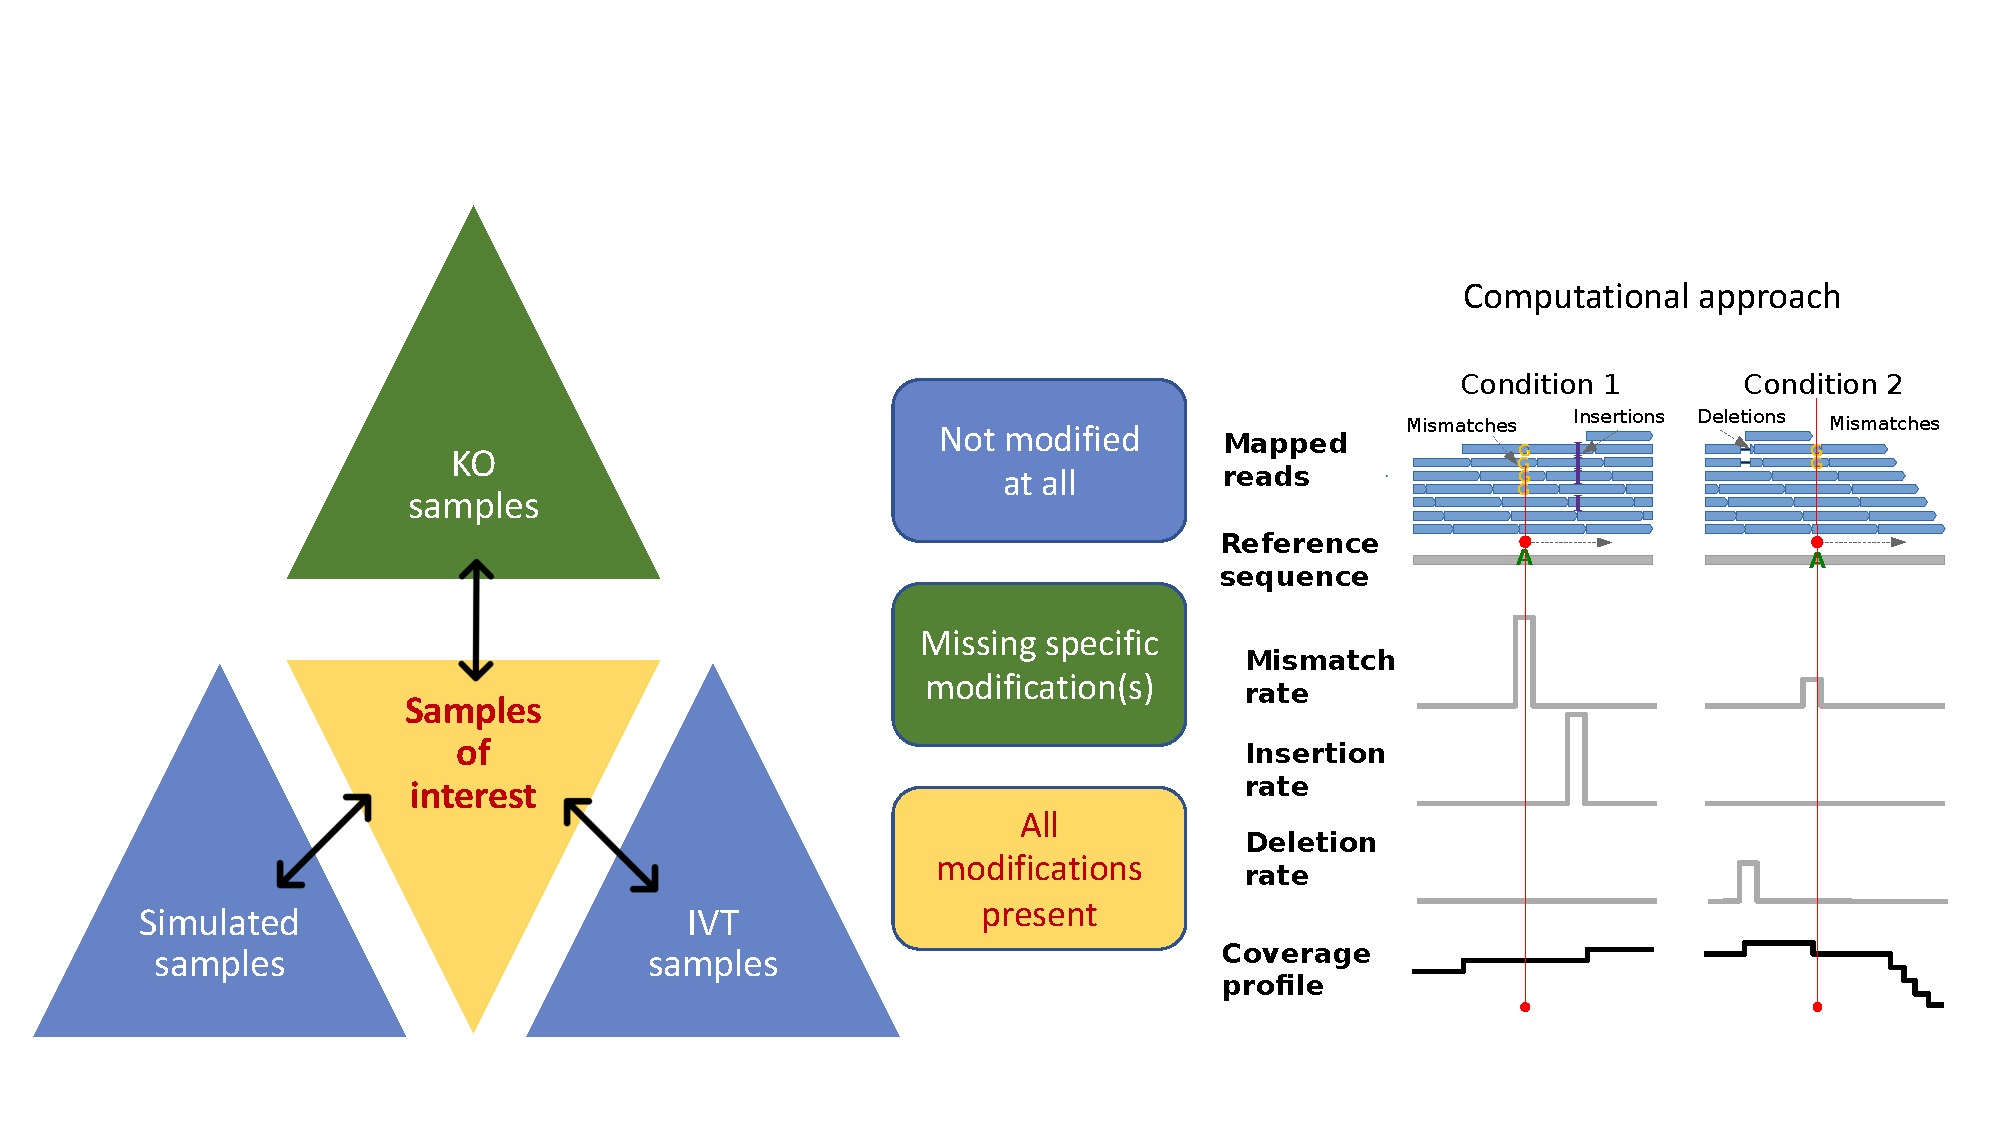
\includegraphics[width = 1\textwidth]{Figure1.pdf}
  \caption{\textbf{General outline of RNA modification detection by JACUSA2.} A key feature of our approach is that multiple replicates can be compared as shown on the left. Samples of interests where all modifications are present could be compared with either KO samples where the modification of interest is missing or IVT/simulated samples where all modifications are absent. Read stacks (in blue) are compared head-to-head as shown on the right. }
  \label{fig:graphicsummary}
      \end{figure}
\newpage

\begin{figure}[h!]
    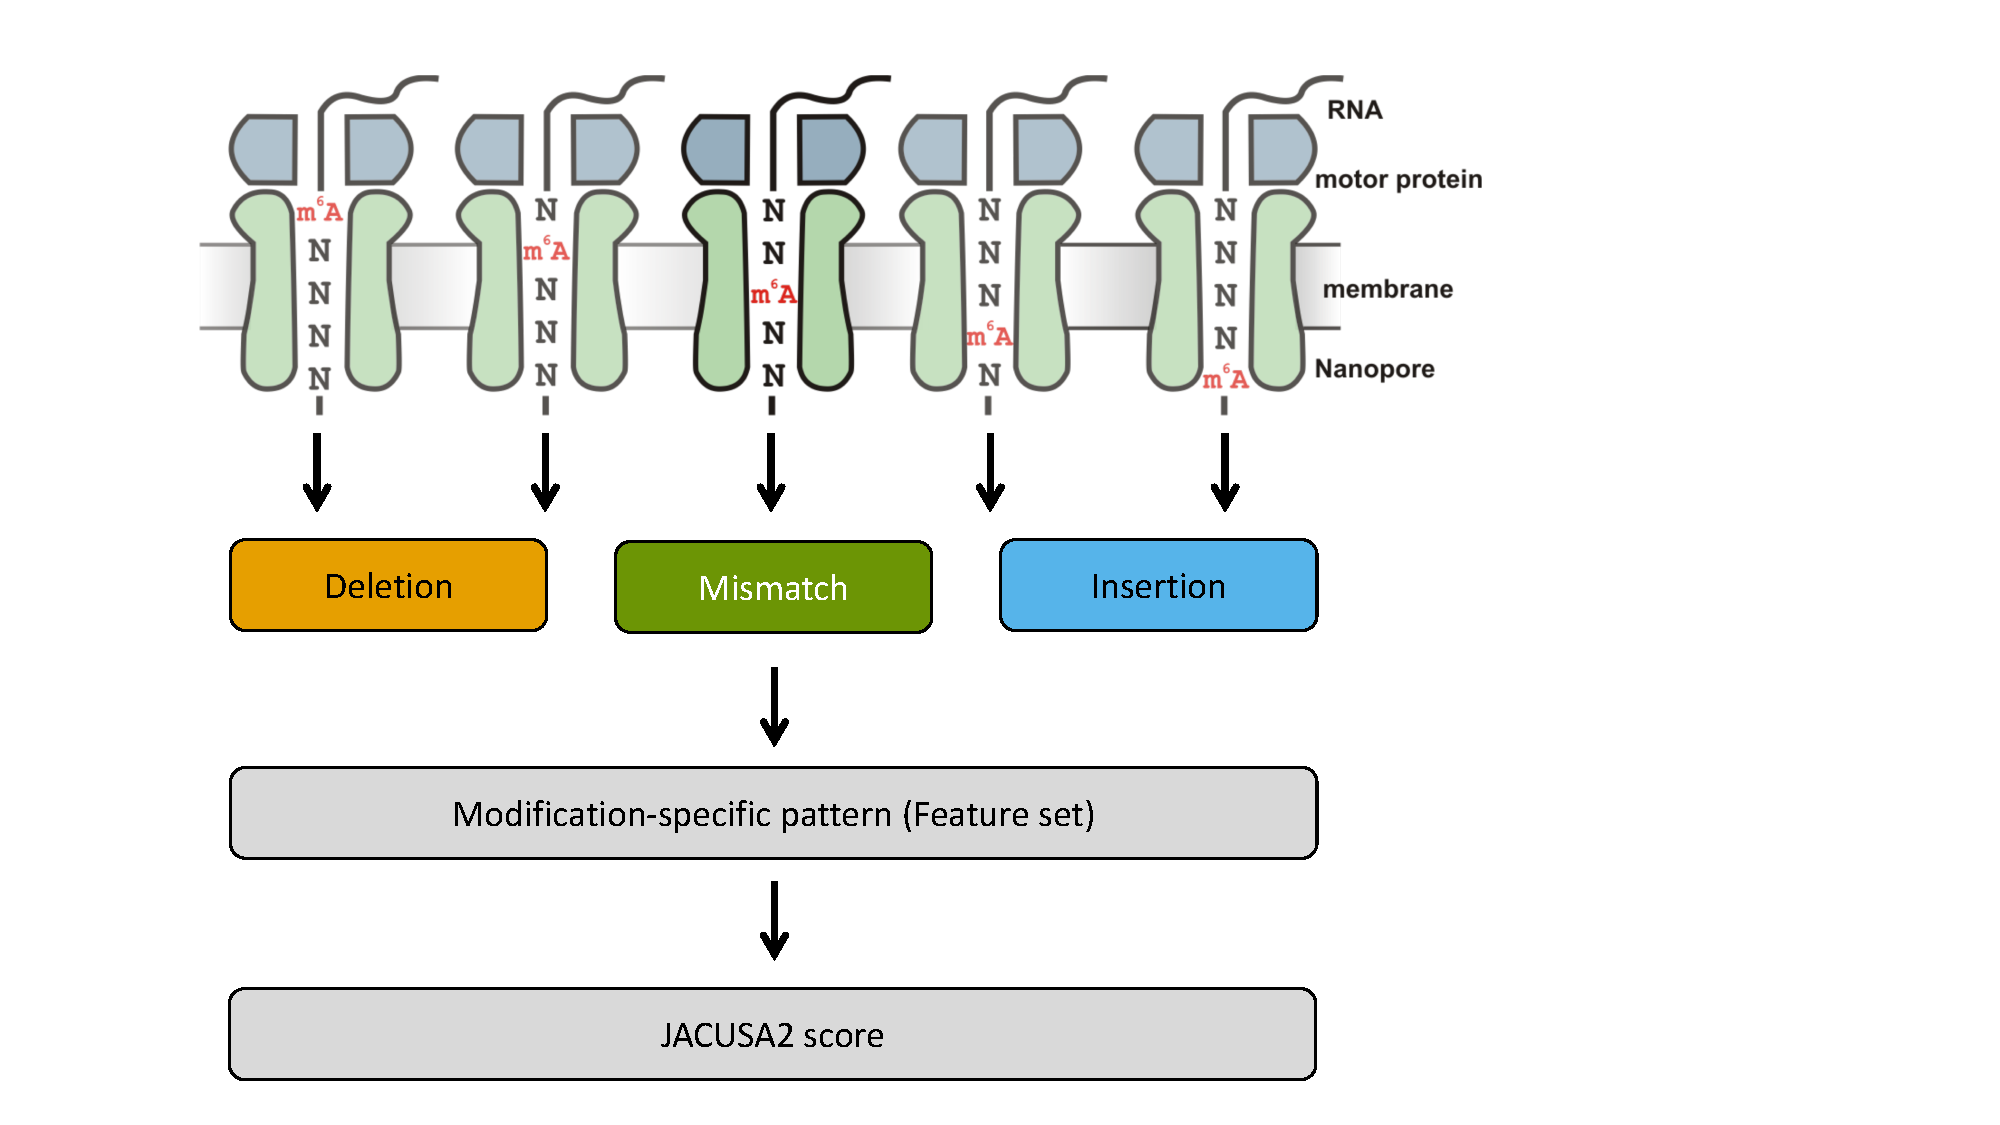
\includegraphics[width = 1\textwidth]{Figure2.pdf}
  \caption{\textbf{Motivation of 5mer context for RNA modification mapping}. The nanopore covers 5 consecutive RNA residues. That is why we consider a 5mer context and derive 3 principal features for every position within a given 5 mer (15 features in total, with a central A residue in this example). We evaluate each feature set by previously learned patterns and compute a final score for modification site detection.}
  \label{fig:5mer}
      \end{figure}
\newpage

\begin{figure}[h!]
    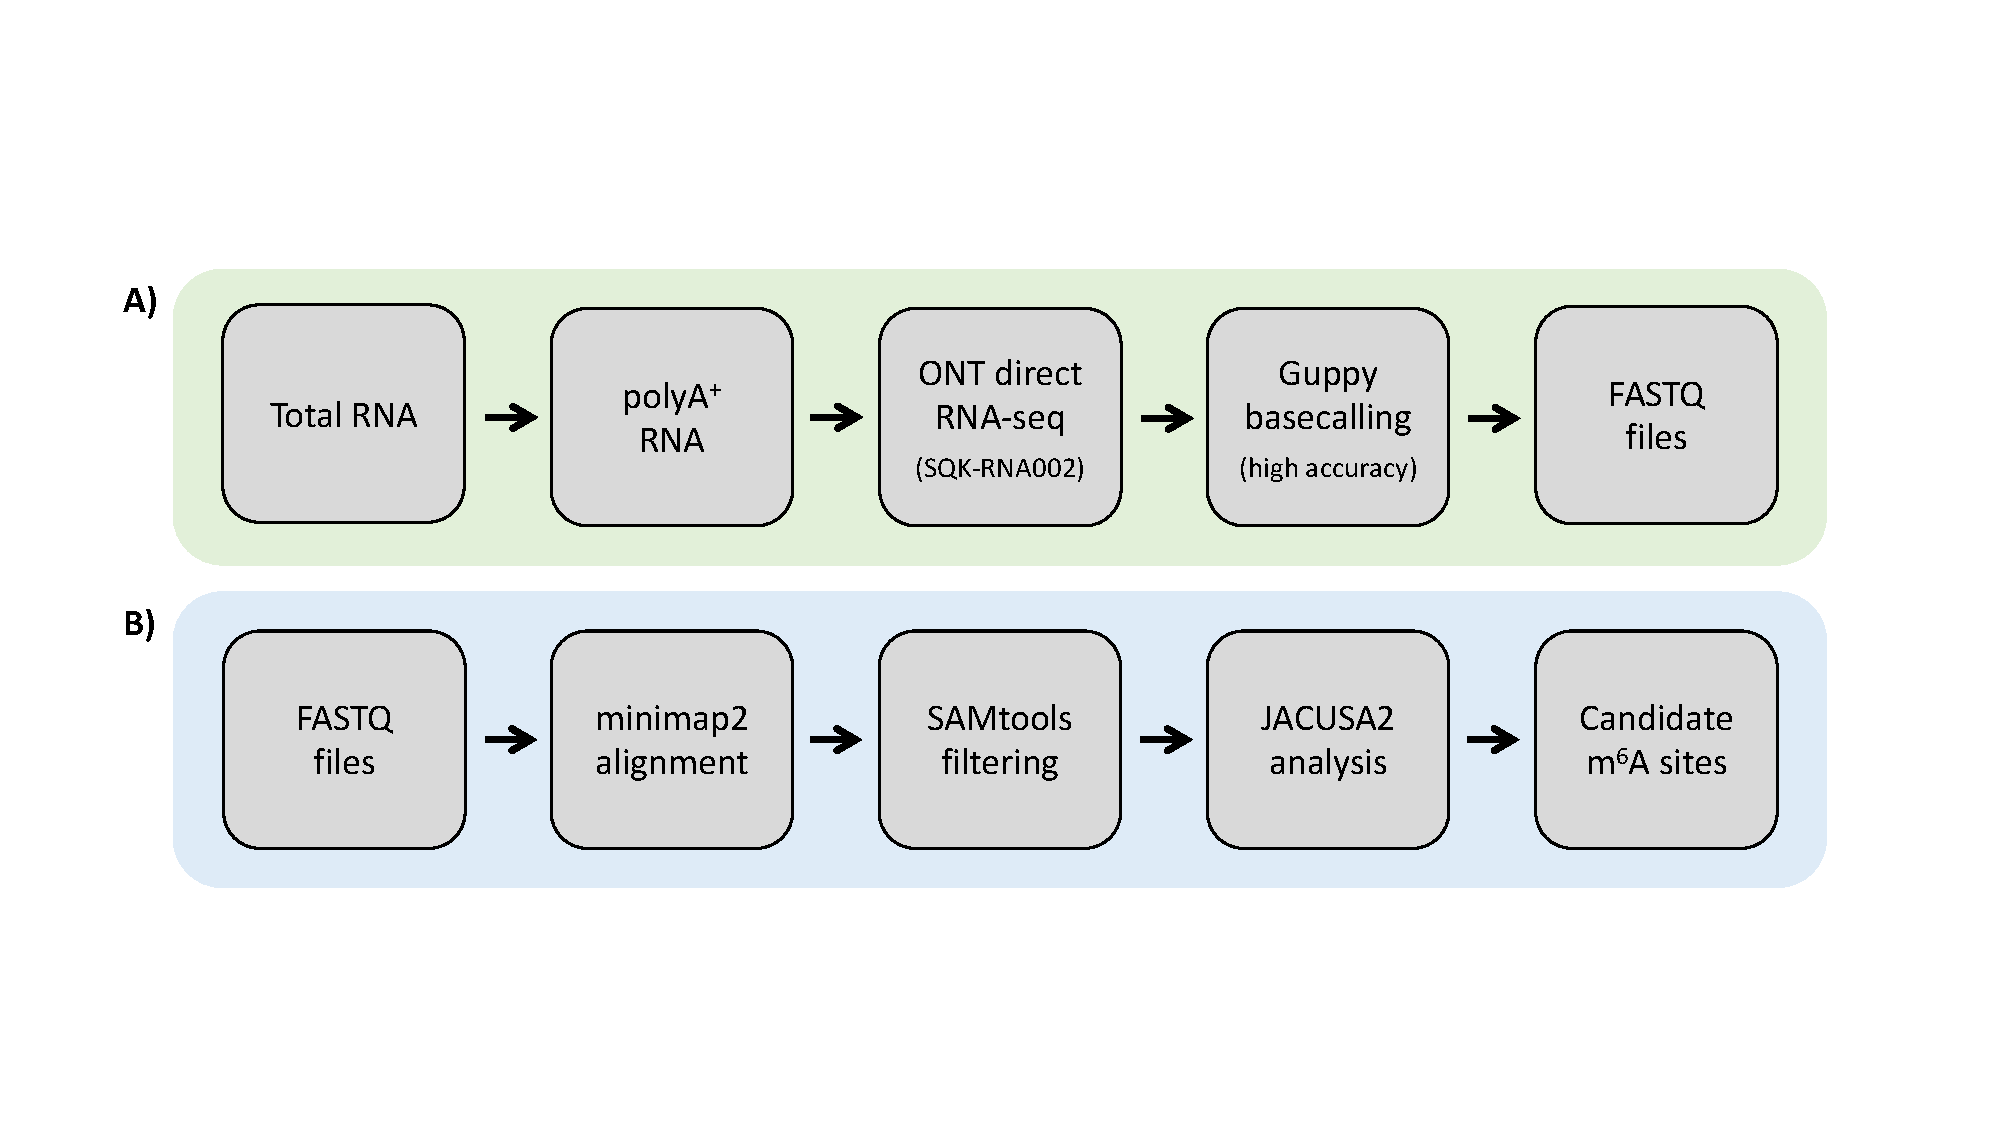
\includegraphics[width = 1\textwidth]{Figure3.pdf}
  \caption{\textbf{Experimental and computational workflow}. tbd}
  \label{fig:workflow}
      \end{figure}
\newpage



\section*{TABLE CAPTIONS}
\section*{TABLES}

\begin{table}[]
\label{tab:software}
\begin{tabular}{|p{1.5cm}|p{7cm}|p{6.5cm}|}
\hline 
            Software & Version & Description \\ 
            \hline \hline
            \texttt{Minimap2} & \url{https://github.com/lh3/minimap2} v2.22 or later & \url{https://lh3.github.io/minimap2/} \\ \hline
            \texttt{samtools} & \url{https://github.com/samtools/samtools} v1.12 or later & \url{http://samtools.github.io/} \\ \hline
	   \texttt{JAVA} & openjdk 11.0.12 2021-07-20 - JAVA 11 or later & OpenJDK Runtime Environment\\ \hline
	   \texttt{R} &  \url{https://www.r-project.org/} version 3.5.1 or later & The R Project for Statistical Computing \\ \hline
	   \texttt{PERL} &  \url{https://www.perl.org/} version 5.28.1 or later & Perl is a highly capable, feature-rich programming language \\ \hline
	   \texttt{BASH, sed, awk} &  should be part of your Linux distribution & Misc.\\ \hline
	   \texttt{bedtools} &  \url{https://github.com/arq5x/bedtools2} version 2.29.2 or later & Perl is a highly capable, feature-rich programming language \\ \hline	   
	   \texttt{NanoSim} &  \url{https://github.com/bcgsc/NanoSim} version 3.0.2 or later (optional) & NanoSim is a fast and scalable read simulator that captures the technology-specific features of ONT data\\ \hline	   
\end{tabular}
\caption{\textbf{Software dependencies}\label{tab:software} blubba}
\end{table}

\begin{table}[]
\label{tab:packages}
\begin{tabular}{|p{1.5cm}|p{7cm}|p{6.5cm}|}
\hline 
            R Packages & Version & Description \\ 
            \hline \hline
            \texttt{ggplot2} & \url{https://cran.r-project.org/web/packages/ggplot2/index.html} - ggplot2\_3.3.0 or later &  ggplot2 is a system for declaratively creating graphics, based on The Grammar of Graphics. \\ \hline
            \texttt{NMF} & \url{https://cran.r-project.org/web/packages/NMF/index.html} - NMF\_0.22.0 or later &  Provides a framework to perform Non-negative Matrix Factorization (NMF). \\ \hline
\end{tabular}
\caption{\textbf{R Package dependencies}\label{tab:software} blubba}
\end{table}



\end{document}
